\documentclass[handout]{beamer}
\usepackage{array}
\usepackage{german}
\usepackage{graphicx}
\usepackage[utf8]{inputenc}
\usepackage[T1]{fontenc}
\mode<beamer>{%
\usetheme{Copenhagen}
}
\usepackage[orientation=landscape,size=a3,debug,scale=2.5]{beamerposter}
\title[]{}
\begin{document}
\begin{frame}
\frametitle{%\hspace{0pt plus 1 filll}
MathSem 2023: Harmonische Analysis}
\begin{columns}[t,onlytextwidth]
\begin{column}{0.32\textwidth}
\begin{center}
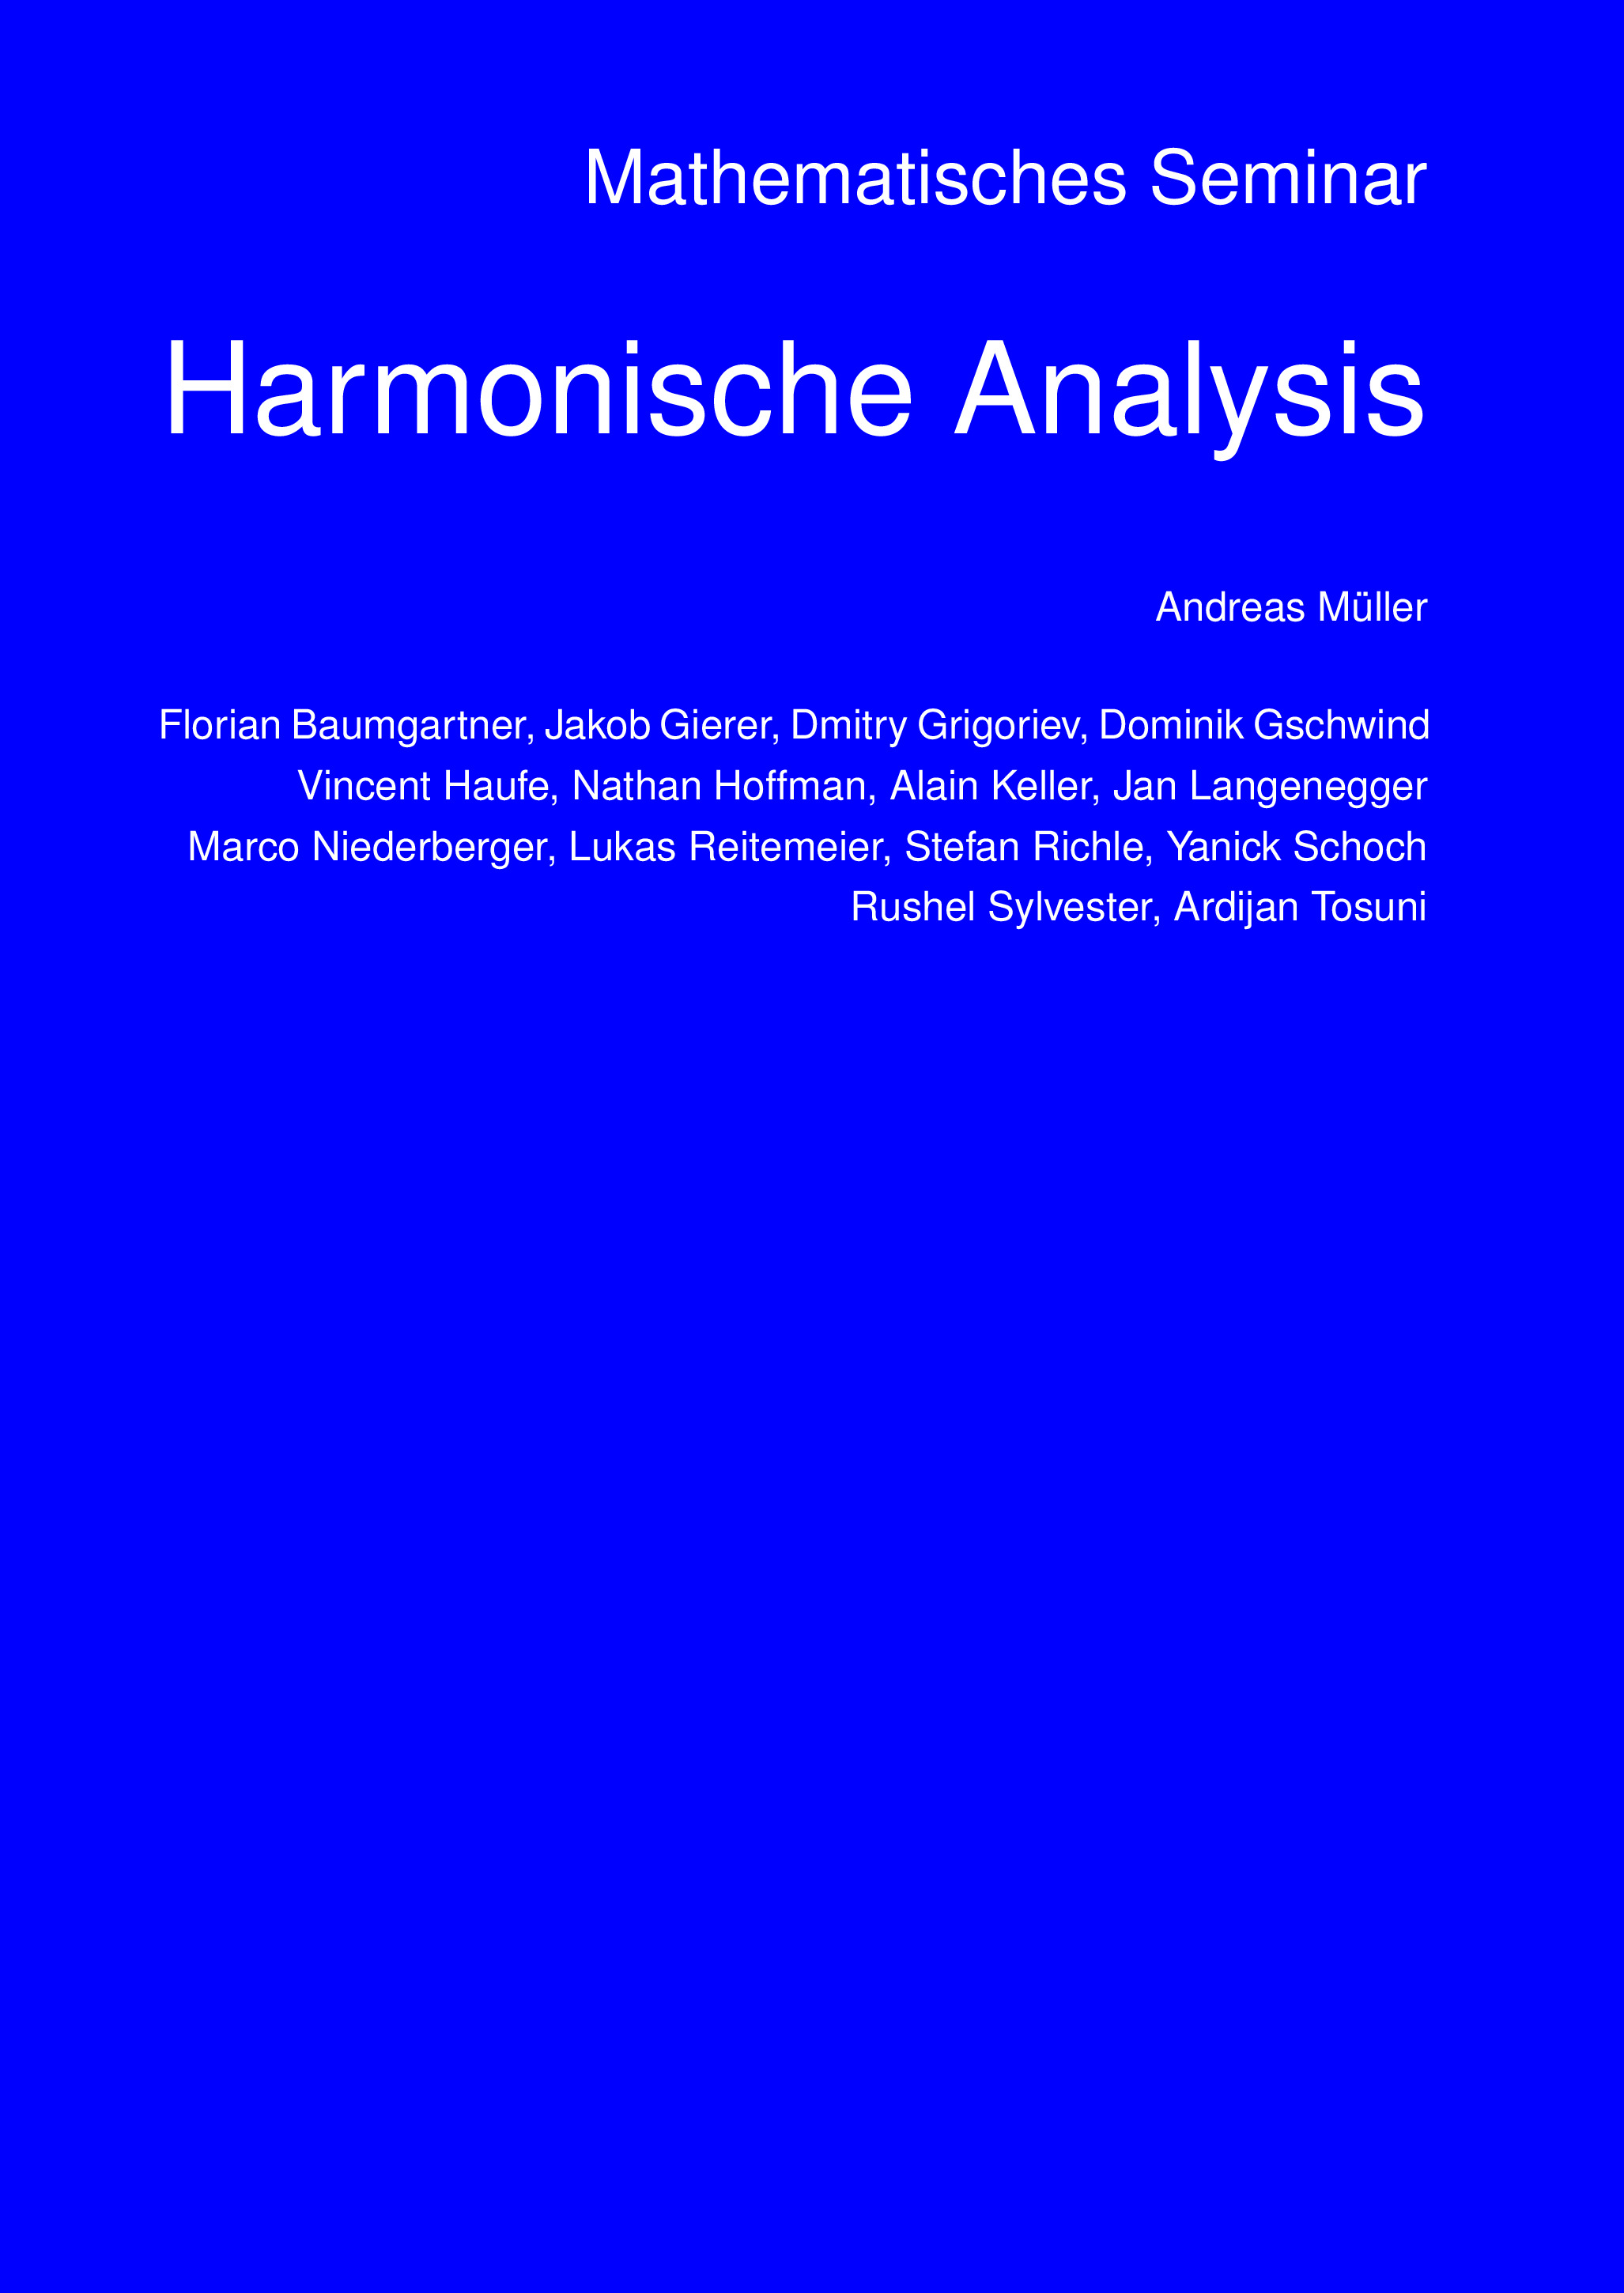
\includegraphics[width=\hsize]{../cover/buchcover.png}
\end{center}
\vskip 0.2cm
\bigskip
\bigskip
Erscheint~im~Herbst~2023.\\
Anfragen~an~Prof.~Dr.~Andreas Müller,\\
{\texttt{andreas.mueller@ost.ch}}
\bigskip
\bigskip
\bigskip
%\vskip 1.2cm
\end{column}
%
\begin{column}{0.65\textwidth}
\begin{description}
\item[Teil 1:] Grundlagen
\begin{enumerate}
\item Skalarprodukte
\item Orthogonale Funktionen
\item Gruppen
\item Operatoren
\item Radon-Transformation
\item Diskrete harmonische Analysis
\item Nichtkommutative harmonische Analysis
\end{enumerate}
\item[Teil 2:] Anwendungen und weiterführende Themen
\begin{enumerate}
\setcounter{enumi}{7}
\item Alain Keller: {\em Sonogramm}
\item Florian Baumgartner: {\em Auto-Tune}
\item Lukas Reitemeier:
{\em Brownsche Bewegung und stochastische Differentialgleichungen}
\item Marco Niederberger und Yanick Schoch:
{\em Optische Fourier-Transformation}
\item Jakob Gierer: {\em Bildkompression}
\item Nathan Hoffman: {\em Rekonstruktion eines CT-Bildes}
\item Vincent Haufe: {\em Mellin-Transformation}
\item David Bättig: {\em Harmonische Analysis der Gezeiten}
\item Dmitry Grigoriev: {\em Spektrale Methoden in der Meteorologie}
\item Jan Langenegger: {\em Milankovi\'c-Zyklen}
\item Dominik Gschwind: {\em Kann ein künstliches neuronales Netzwerk
die Fourier-Transformation lernen?}
\item Stefan Richle: {\em Wavelets}
\end{enumerate}
\end{description}
\end{column}
\begin{column}{0.01\textwidth}
\llap{\raisebox{-3cm}{
\includegraphics{qrcode.pdf}}}
\end{column}
\end{columns}
\end{frame}
\end{document}
